% !TeX spellcheck = en_US
\documentclass{beamer}
%\documentclass[handout]{beamer}
\usepackage[english]{babel}
\usepackage[utf8]{inputenc}
\usepackage{graphicx}
\usepackage{amsmath}
\usepackage{tikz}
\usepackage{multirow}
%\usepackage{tcolorbox}
\usefonttheme{structuresmallcapsserif}
\usetheme{Antibes}

\usecolortheme{whale}

\setbeamertemplate{footline}[frame number]

%\usepackage[table, dvipsnames]{xcolor}

\newcommand{\sm}[0]{$M_\odot$}
\newcommand{\erf}[1]{\text{erf}\left(#1\right)}
\def\checkmark{\tikz\fill[scale=0.4](0,.35) -- (.25,0) -- (1,.7) -- (.25,.15) -- cycle;} 

%\usepackage{default}

%\newcounter{stepsBarnes}
%\newcommand{\seti}{\setcounter{stepsBarnes}{\value{enumi}}}
%\newcommand{\conti}{\setcounter{enumi}{\value{stepsBarnes}}}
%\definecolor{green}{RGB}{0, 150, 0}

\begin{document}
\begin{frame}
	\centering
%	\color{white}
	\textsc{\LARGE Orbits of black holes in triaxial potentials}
	\\
	\vspace{2.5cm}
	Juan Barbosa\\
	\vspace{1cm}
	\footnotesize
	Departamento de F\'isica\\
	Facultad de Ciencias\\
	Universidad de los Andes
\end{frame}

\section{Introduction}
\begin{frame}{Introduction}
	\begin{columns}
		\begin{column}{0.5\textwidth}
			\begin{figure}[h]
				\centering
				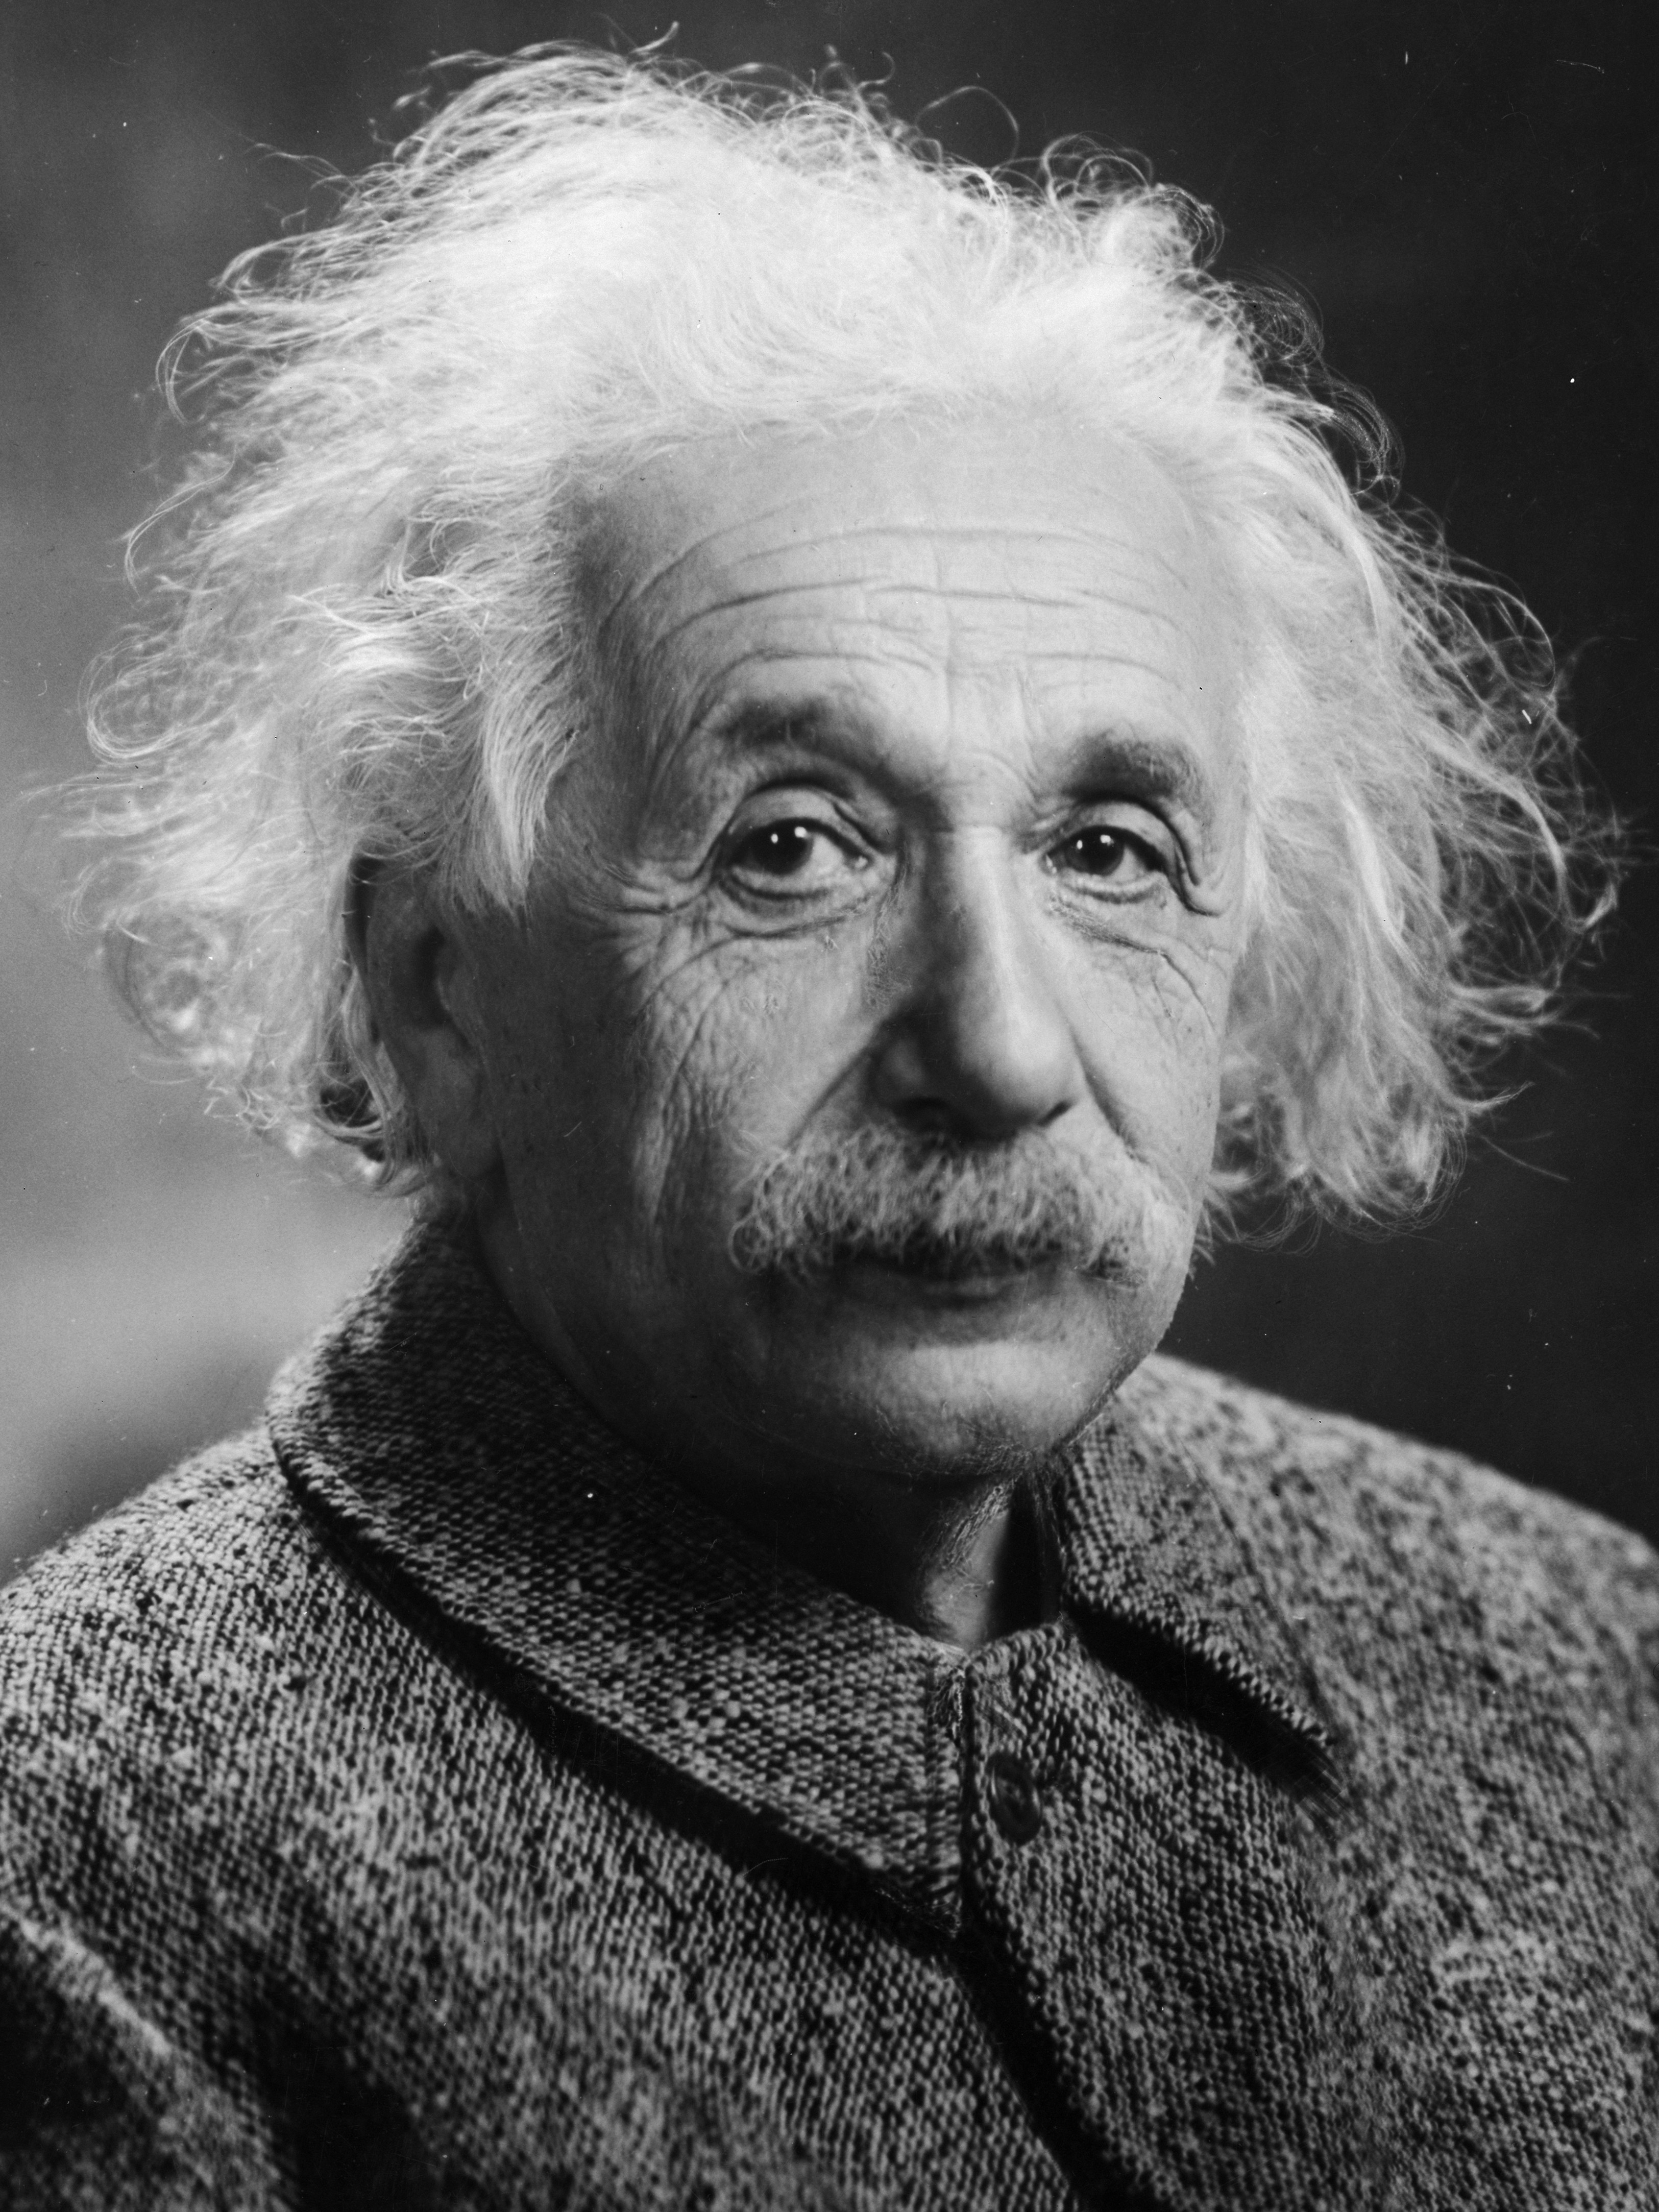
\includegraphics[width=0.9\linewidth]{images/Albert_Einstein_Head}
			\end{figure}
		\end{column}
		\begin{column}{0.5\textwidth}
			\begin{itemize}
				\item Theory of General Relativity, 1906
				\item Although more than 100 years have passed since the publication of the theory, even today there are gaps in the understanding and implications of Einstein's equations
			\end{itemize}
		\end{column}
	\end{columns}
\end{frame}

\begin{frame}{Introduction}
	\begin{figure}
		\centering
		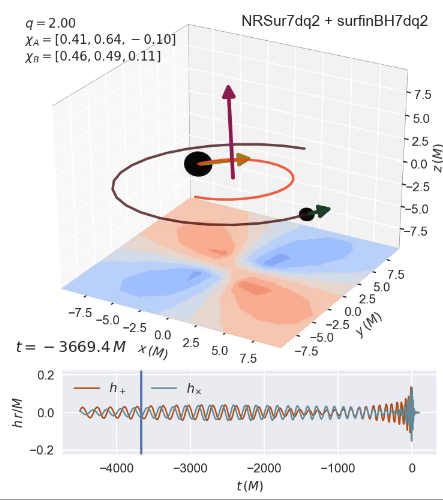
\includegraphics[width=0.4\linewidth]{images/example}
	\end{figure}
	\href{run:/home/juan/Documents/TesisFisica/Slides/images/super_kick.mp4}{Binary black hole explorer}
\end{frame}

\begin{frame}{Objectives}
	\small
	Study the effect of different triaxial potentials, initial speeds and numerical integrators on the times required by a supermassive black hole to return to its initial position, after experiencing a recoil, as well as to quantify how chaotic its trajectory is.
	
	\begin{itemize}
		\item Obtain probability distributions for the return times based on each of the free parameters of the triaxial potential, the magnitude and direction of the initial velocity
		\item Quantify how chaotic is the trajectory of the black hole in each simulation, using exponents of Lyapunov
		\item Evaluate the performance of the numerical integrators using the information of the simulations
	\end{itemize}
\end{frame}

\section{Methodology}
\subsection{Units}
\begin{frame}{Methodology}
	Computer simulations are sensitive to rounding errors due to the lack of infinite precision when representing decimal numbers.
	\begin{figure}[h]
		\centering
		\includegraphics[width=0.7\linewidth]{"../Files/Week 3/floating"}
		\caption{Floating point precision for different values, for a 32 bit and 64 bit holders.}
		\label{fig: IEEE-754}
	\end{figure}
\end{frame}

\begin{frame}{}
	\begin{table}[h]
		\centering
		\caption{Units of measure used on the simulations.}
		\label{tb: units}
		\begin{tabular}{c|c}
			\hline
			\textbf{Physical property} & \textbf{unit} \\
			\hline
			Length & 1 kilo-parsec (kpc) \\
			Mass & $10^5$ solar masses ($10^5$ \sm) \\
			Time & 1 giga-year (Gyr) \\
			\hline
		\end{tabular}
	\end{table}
	\begin{enumerate}
		\item Universal gravitational constant:
		\begin{equation}
			G = 0.4493 \quad \dfrac{\text{kpc$^3$}}{\text{Gy$r^210^5$\sm}}
		\end{equation}
		\item Hubble parameter:
			\begin{equation}
			H \approx 1.023 H_0 \times10^{-3} \text{ Gyr$^{-1}$} = 6.916\times10^{-2}\text{ Gyr$^{-1}$}
			\end{equation}
	\end{enumerate}
\end{frame}

\begin{frame}
	Mass distributions of the host galaxy, are divergent. The end of the host is taken at the virial radius.
	\begin{equation}\label{eq: critical_density}
		\rho_\text{crit} = \dfrac{3H(t)^2}{8\pi G}
	\end{equation}
	
	\begin{equation}\label{eq: R_vir_def}
		\dfrac{M(R_\text{vir})}{V(R_\text{vir})} = \bar{\rho}(R_\text{vir}) =  200 \rho_\text{crit} = 75\dfrac{H(t)^2}{\pi G}
	\end{equation}
	where $M(R_\text{vir})$ is the cumulative mass, and $V(R_\text{vir})$: the volume
\end{frame}

\subsection{Equation of motion}
\begin{frame}{}
Trajectories of the kicked black holes are obtained by numerically solving the equation of motion.
\begin{equation}\label{eq: equationMotion}
	\ddot{\vec{x}} = -a_\text{grav}(\vec{x})\hat{x} + \left(a_\text{DF}(\vec{x}, \dot{\vec{x}})-\dot{x}\dfrac{\dot{M_\bullet}(x, \dot{x})}{M_\bullet}\right)\dot{\hat{x}} 
\end{equation}

where $M_\bullet$ is the black hole mass
\end{frame}

\begin{frame}{Dynamical friction}
	As the black hole travels through the galaxy, dark matter, stars and gaseous materials from the medium interact with the black hole adding a drag force due to friction. 
	\begin{equation}\label{eq: df_cl}
		a_\text{DF}^\text{cl}(\vec{x}, \dot{\vec{x}}) = -\dfrac{4\pi G^2}{\dot{x}^2} M_\bullet\rho(\vec{x})\ln\Lambda\left(\erf{X} - \dfrac{2}{\sqrt{\pi}}Xe^{-X^2}\right)
	\end{equation}
%	\begin{equation}
%		\rho(\vec{x}) = \rho_\text{DM}(\vec{x}) + \rho_\text{stars}(\vec{x})
%	\end{equation}
	\begin{equation}
	X \equiv \dfrac{|\dot{x}|}{\sqrt{2}\sigma_\text{DM}} \qquad \text{with } \sigma_\text{DM} = \sqrt{\dfrac{GM_\text{DM}}{2R_\text{vir}}}
	\end{equation}
\end{frame}

\begin{frame}
	Drag generated by gas depends on local sound speed
	\begin{equation}
		\mathcal{M}(\dot{x}) \equiv \dfrac{|\dot{x}|}{c_s} = |\dot{x}|\sqrt{\dfrac{\mathcal{M}_w}{\gamma RT_\text{vir}}} = |\dot{x}|\sqrt{\dfrac{\mathcal{M}_w}{\gamma R}\left(\dfrac{2k_BR_\text{vir}}{\mu m_p G M_h}\right)}
	\end{equation}
	\begin{equation*}
		\mathcal{M}(\dot{x}) = 1.63|\dot{x}|\sqrt{\dfrac{R_\text{vir}}{M_h}}
	\end{equation*}
	
	\begin{equation}\label{eq: df_c}
	a^\text{c}_\text{DF}(\vec{x}, \dot{\vec{x}}) = -\dfrac{4\pi G^2}{\dot{x}^2}M_\bullet\rho_\text{gas}(\vec{x})f(\mathcal{M})
	\end{equation}
	
	with
	\begin{equation}\footnotesize
	f(\mathcal{M}) = \left\{
	\begin{matrix}
	0.5\ln\Lambda \left[\erf{\dfrac{\mathcal{M}}{\sqrt{2}}} - \sqrt{\dfrac{2}{\pi}}\mathcal{M}e^{-\mathcal{M}^2/2}\right]& \text{if $\mathcal{M} \leq 0.8$}\\
	1.5\ln\Lambda \left[\erf{\dfrac{\mathcal{M}}{\sqrt{2}}} - \sqrt{\dfrac{2}{\pi}}\mathcal{M}e^{-\mathcal{M}^2/2}\right] & \text{if $0.8 < \mathcal{M} \leq \mathcal{M}_{eq}$}\\
	0.5\ln\left(1 - \mathcal{M}^{-2}\right) + \ln\Lambda & \text{if $\mathcal{M} > \mathcal{M}_{eq}$}
	\end{matrix}
	\right.
	\end{equation}
\end{frame}

\begin{frame}{Accretion into the black hole}
	As the black hole accretes matter from the surroundings, an acceleration appears, due to the second law of Newton.
	\begin{equation}
		\dot{M}_\bullet(\vec{x}, \dot{\vec{x}}) = \left\{
		\begin{array}{lc}
		\dot{M}_\bullet^\text{BHL}(\vec{x}, \dot{\vec{x}}) & \text{if $\dot{M}_\bullet^\text{BHL} < \dot{M}_\bullet^\text{Edd}$} \\
		\dot{M}_\bullet^\text{Edd} & \text{else}
		\end{array}
		\right.
	\end{equation}
	
	\begin{equation}
		\dot{M}_\bullet^\text{BHL}(\vec{x}, \dot{\vec{x}}) = \dfrac{4\pi G^2 \rho_G(\vec{x})M^2_\bullet}{\left(c_s^2 + \dot{x}^2\right)^{3/2}} % \qquad \text{with } \rho_B(\vec{x}) = \rho_\text{stars}(\vec{x}) + \rho_\text{gas}(\vec{x})
	\end{equation}
	\begin{equation}
		\dot{M}_\bullet^\text{Edd} = \dfrac{(1 - \epsilon)M_\bullet}{\epsilon t_\text{Edd}} \qquad \epsilon = 0.1, \quad t_\text{Edd} = 0.44 \text{ Gyr}
	\end{equation}
\end{frame}

\section{Studies}
\begin{frame}{Spherical case}
	\begin{figure}[h]
		\centering
		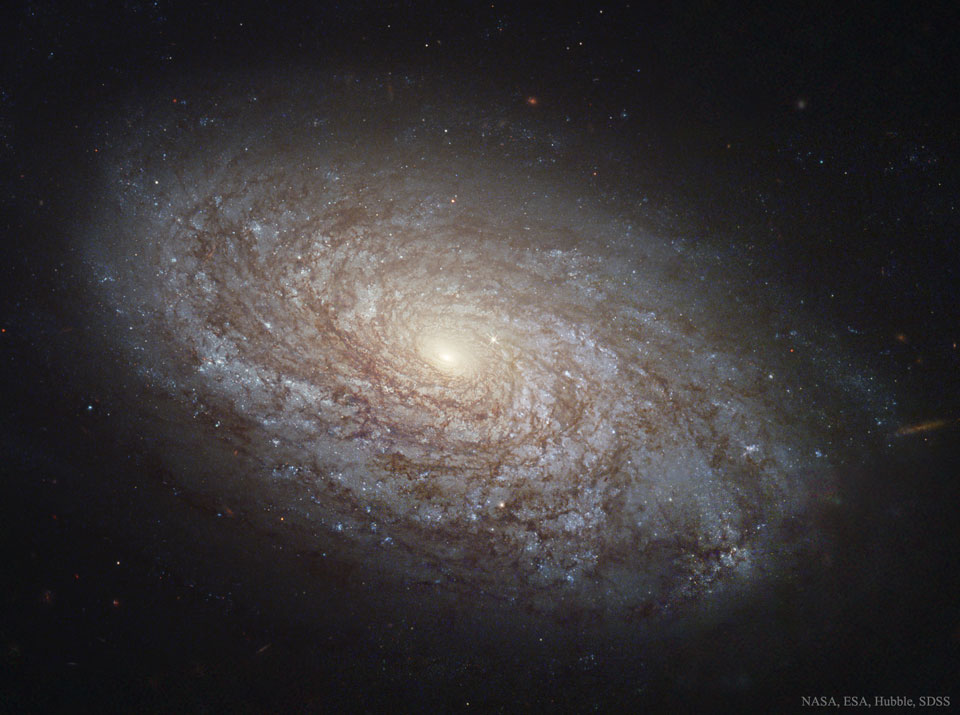
\includegraphics[width=0.8\linewidth]{../Documento/Figures/NGC4414_modified}
		\caption{NGC4414 galaxy as seen by the Hubble telescope.}
	\end{figure}
\end{frame}

\begin{frame}
	Mass distribution between components is given by:
	\begin{equation}
		M_\text{DM}(R_\text{vir}) = (1 - f_b)M_h
	\end{equation}
	\begin{equation}
		M_\text{stars}(R_\text{vir}) = f_sf_bM_h
	\end{equation}
	\begin{equation}
		M_\text{gas}(R_\text{vir}) = (1 - f_s)f_bM_h
	\end{equation}
	
	with $f_b = 0.156$ and $M_h = 10^8$ \sm
	\begin{equation}
		R_\text{vir} = \left({\dfrac{M_hG}{100 H(t)^2}}\right)^{1/3}
	\end{equation}
\end{frame}

\begin{frame}
	\begin{enumerate}
		\item Dark matter (NWF):
		\begin{equation}\label{eq: dmdensity}
			\rho_\text{DM}(r) = \dfrac{\rho_0^\text{DM}}{\frac{r}{R_s}\left(1 + \frac{r}{R_s}\right)^2}
		\end{equation}
		\item Stellar density (Hernquist):
		\begin{equation}
			\rho_s(r) = \dfrac{f_sf_bM_h \mathcal{R}_s}{2\pi r(r + \mathcal{R}_s)^3}
		\end{equation}
		\item Gas density (Power law):
		\begin{equation}
			\rho_\text{gas}(r) = \left \{
			\begin{matrix}
			\rho_0^\text{gas} & \text{if $r < r_0$}\\
			\rho_0^\text{gas}\left(\dfrac{r_0}{r}\right)^{-n} & \text{if $r \geq r_0$}\\
			\end{matrix}
			\right.
		\end{equation}
	\end{enumerate}
\end{frame}


\subsection{Results}
\begin{frame}
	\begin{figure}[h]
		\centering
		\includegraphics[height=0.9\textheight]{"../Files/Week 6/properties_s01v70"}
		\caption{Properties of a single simulation.}
	\end{figure}
\end{frame}

\begin{frame}
	\begin{figure}[h]
		\centering
		\includegraphics[width=0.9\linewidth]{"../Files/Week 6/returntimes_stellar_speed"}
		\caption{Return time for different stellar densities.}
	\end{figure}
\end{frame}

\begin{frame}
\begin{figure}[h]
	\centering
	\includegraphics[width=0.9\linewidth]{"../Files/Week 6/mass_stellar_speed"}
	\caption{Black holes mass as function of initial speed and stellar fraction.}
\end{figure}
\end{frame}

\begin{frame}
\begin{figure}[h]
	\centering
	\includegraphics[width=0.9\linewidth]{"../Files/Week 6/mass_stellar_speed_2"}
	%	\caption{NGC4414 galaxy as seen by the Hubble telescope.}
\end{figure}
\end{frame}
\begin{frame}
\begin{figure}[h]
	\centering
	\includegraphics[width=0.9\linewidth]{"../Files/Week 6/mass_stellar_speed_3"}
%	\caption{NGC4414 galaxy as seen by the Hubble telescope.}
\end{figure}
\end{frame}

\begin{frame}{Schedule}
	\begin{table}[h]
		\centering
		\caption{Activity schedule}
		\label{tb: cronograma}
		\tiny
		\begin{tabular}{|c|c|c|c|c|c|c|c|c|c|c|c|c|c|c|c|c|}
			\hline
			& \multicolumn{16}{c|}{\textbf{Week}} \\ \cline{2-17} 
			\multirow{-2}{*}{\textbf{Activities}} & \textbf{1} & \textbf{2} & \textbf{3} & \textbf{4} & \textbf{5} & \textbf{6} & \textbf{7} & \textbf{8} & \textbf{9} & \textbf{10} & \textbf{11} & \textbf{12} & \textbf{13} & \textbf{14} & \textbf{15} & \textbf{16} \\ \hline
			\textbf{Task 1} & x & & & & & & & & & & & & & & & \\ \hline
			\textbf{Task 2} & x & x & & & & & & & & & & & & & & \\ \hline
			\textbf{Task 3} & & x & x & x & & & & & & & & & & & & \\ \hline
			\textbf{Task 4} & & & & & x & x & & & & & & & & & & \\ \hline
			\textbf{Task 5} & & & & & & & x & & & & & & & & & \\ \hline
			\textbf{Task 6} & & & & & & & & x & x & & & & & & & \\ \hline
			\textbf{Task 7} & & & & & & & & & & x & x & x & & & & \\ \hline
			\textbf{Task 8} & & & & & & & & & & & & & x & x & x & x \\ \hline
		\end{tabular}
	\end{table}
	\begin{itemize}
		\footnotesize
		\item \textbf{Task 1:} REBOUND instalaci\'on in HPC \checkmark
		\item \textbf{Task 2:} Understanding REBOUND examples \checkmark
		\item \textbf{Task 3:} Implementation of a Choksi simulation \checkmark
		\item \textbf{Task 4:} Implementation of a triaxial simulation
		\item \textbf{Task 5:} 30 \% thesis dissertation
		\item \textbf{Task 6:} Optimization of the time step for \textit{WHFast} y \textit{IAS15}
%		\item \textbf{Task 7:} Implementaci\'on de un algoritmo automatizado para barrer el espacio de par\'ametros de velocidades iniciales y par\'ametros del potencial triaxial, para los integradores \textit{Leapfrog, WHFast} y \textit{IAS15}
%		\item \textbf{Task 8:} An\'alisis de resultados y escritura de la monograf\'ia
	\end{itemize}
\end{frame}
\end{document}